\chapter{Приложение 1. Результаты экспериментов}

\begin{table}[h]%
    \caption{Значения коэффициентов параметров ARIMAX(2, 0, 3)x(0, 1, 1, 7) с экзогенными переменными: индикатор дня недели и индикатор Рождества}
    \centering
    \begin{tabular}{|l|r||r|r|}
        \hline
            Параметр           &     Значение коэффициента  &  Дисперсия  &  P-value \\
        \hline
            intercept          &     3.7294                 &     1.686 &   0.027 \\
            Friday             &     0.0159                 &  2440.530 &   1.000 \\
            Monday             &     0.0045                 &  5202.932 &   1.000 \\
            Saturday           &    -0.0011                 &  7994.566 &   1.000 \\
            Sunday             &     0.0055                 &  4295.359 &   1.000 \\
            Thursday           &    -0.0069                 &  5951.614 &   1.000 \\
            Tuesday            &    -0.0007                 &  7381.431 &   1.000 \\
            Wednesday          &     0.0078                 &  3557.219 &   1.000 \\
            xmas               & -8738.4506                 &   399.352 &   0.000 \\
            ar.L1              &     0.0149                 &     0.067 &   0.824 \\
            ar.L2              &     0.8291                 &     0.056 &   0.000 \\
            ma.L1              &     0.3286                 &     0.074 &   0.000 \\
            ma.L2              &    -0.5438                 &     0.062 &   0.000 \\
            ma.L3              &    -0.1352                 &     0.038 &   0.000 \\
            ma.S.L7            &    -0.9363                 &     0.017 &   0.000 \\
            sigma2             &  1.264e+06                 &  3.87e+04 &   0.000 \\
        \hline
    \end{tabular}
    \label{tbl:arimax_coeffs_exogen}
\end{table}


\def\figurename{Рис}
\begin{figure}[h]
	\centering
	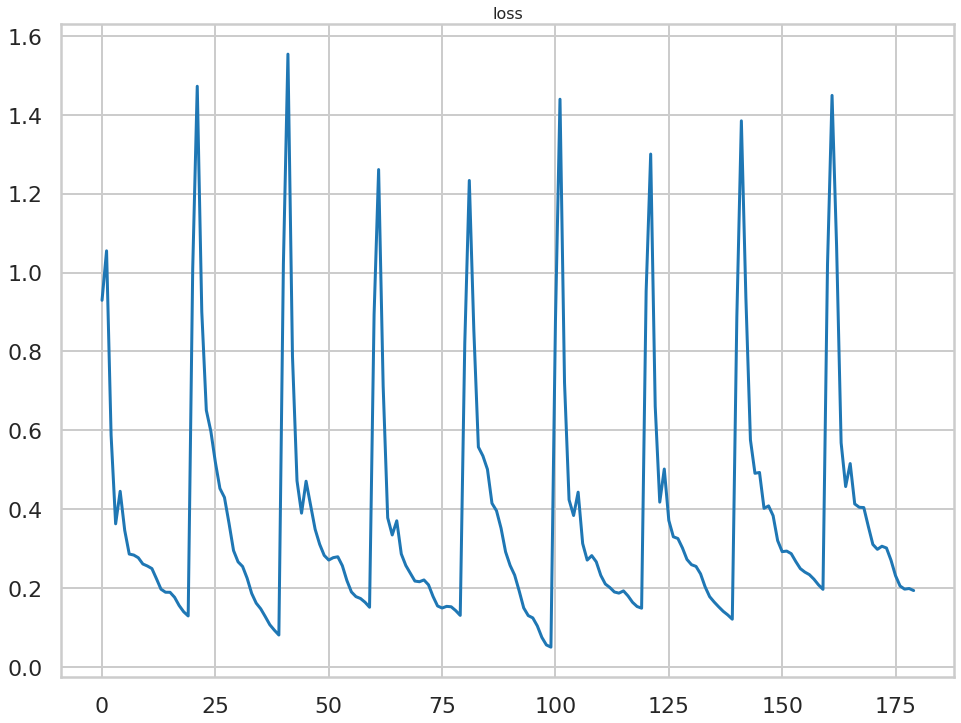
\includegraphics[height=10cm]{./img/fcm_losses.png}
	\caption{Графики значений функции потерь для FCM-LSTM. Каждый концепт обучался 20 эпох.}
	\label{img:fcm_losses}
\end{figure}

\begin{figure}[h]
	\centering
	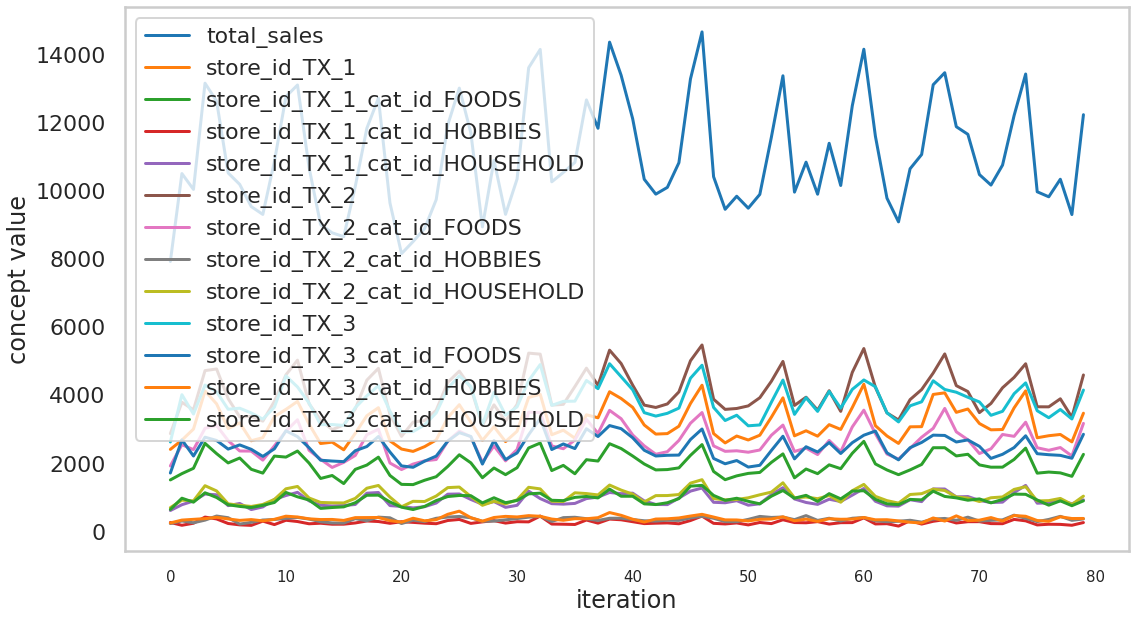
\includegraphics[height=10cm]{./img/plot_concept_history.png}
	\caption{Результат работы метода plot\_concept\_history для карты, обученной на 80 точках исследуемых данных.}
	\label{img:plot_concept_history}
\end{figure}